\subsection{Câmeras}
    \label{subsec:intro_cam}
Para a aquisição de imagens, uma câmera é posicionada no mundo com um ponto de referência
% , conforme ilustrado na Figura~\ref{fig:intro_cam_coord}
. Dessa forma, por semelhança de triângulos, a projeção $\mathbf{P}$ de pontos 3D do mundo em pontos 2D da imagem corresponde a $(x, y, z) \to (f \frac{X}{Z}, f \frac{Y}{Z}, f) = (f \frac{X}{Z}, f \frac{Y}{Z})$, ou seja, $\mathbf{P} \mathbf{X} = \mathbf{x}$.

% \begin{figure*}[!ht]
%     \begin{center}
%         \bmvaHangBox{\fbox{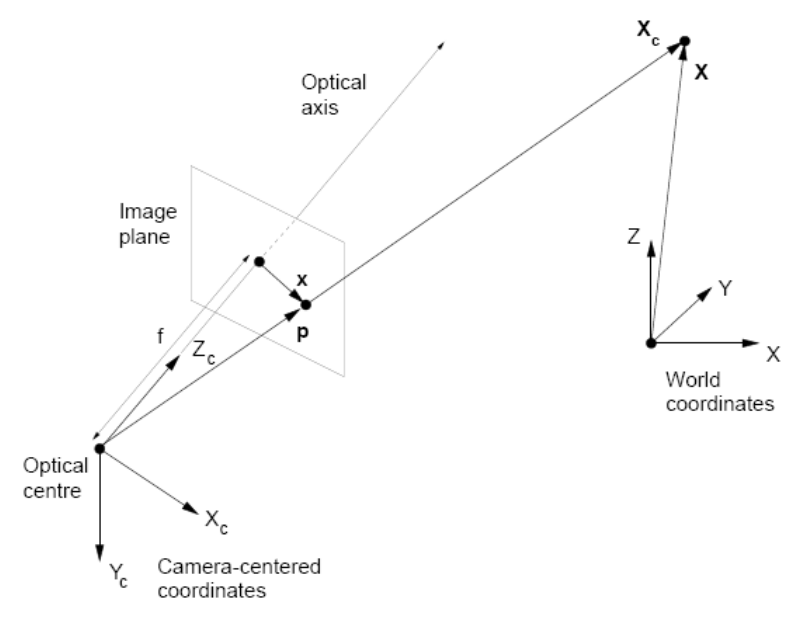
\includegraphics[width=5cm]{Figs/Introducao/cam_coord.png}}}
%     \end{center}
%     \caption{Localização e relação das coordenadas da câmera com a do mundo. Fonte~\cite{FergusL1}.}
%     \label{fig:intro_cam_coord}
% \end{figure*}

A projeção $\mathbf{P}$ é a combinação de três transformações de coordenadas:~\emph{matriz de intrínsecos} $\mathbf{K}$ (posicionamento do ponto focal e do ponto principal, ângulo entre eixos e outros), matriz de projeção $[\mathbf{I} ~|~ \mathbf{0} ]$ e~\emph{matriz de extrínsecos} $[\mathbf{R} ~|~ \mathbf{t} ]$ (relação entre as coordenadas da câmera e os~\emph{pixels})~\cite{FergusL1}.

% , onde:
% $$
%     {\mathbf{K}}
%     =
%     \begin{bmatrix} 
%         f_x & \alpha & c_x\\
%         0 & f_y & c_y \\
%         0 & 0 & 1 \\
%     \end{bmatrix}
%     =
%     \begin{bmatrix} 
%         \text{dist. focal em~\emph{pixels} hor.} & \text{âng. entre eixos} & \text{centro hor.} \\
%         0 & \text{dist. focal em~\emph{pixels} ver.} & \text{centro ver.} \\
%         0 & 0 & 1 \\
%     \end{bmatrix}
%     .
% $$